\chapter{Short Read Structural Variation Detection and Characterization Using Convolutional Neural Networks}

\section{Introduction}

Genomic structural variation, broadly defined as genetic polymorphisms larger than 50bp, are an increasingly prevalent area of study in medical, agricultural, and ecological contexts \cite{sudmantIntegratedMapStructural2015,duAnalysisStructuralVariants2021,weissensteinerDiscoveryPopulationGenomics2020,chakrabortyEvolutionGenomeStructure2021,chakrabortyHiddenGeneticVariation2018,merkerLongreadGenomeSequencing2018,bickhartChallengesImportanceStructural2014}. Structural variation has traditionally been a difficult aspect of the genome to detect and characterize with commonly used short-read sequencing approaches, though a variety of methods have been developed in attempt to increase detection power \cite{clealDysguEfficientStructural2022,rauschDELLYStructuralVariant2012,chenMantaRapidDetection2016,belyeuSamplotPlatformStructural2021,popicCueDeeplearningFramework2023}(reviewed in \cite{cameronComprehensiveEvaluationCharacterisation2019}, \cite{mahmoudStructuralVariantCalling2019} and \cite{alkanGenomeStructuralVariation2011}). Long-read genome sequencing methods have become the \textit{de facto} approach for highly accurate structural variant calling but remain a relatively expensive and low-throughput method compared to short-read sequencing \cite{merkerLongreadGenomeSequencing2018,dierckxsensBenchmarkStructuralVariation2021,chenDecipheringExactBreakpoints2023,ahsanSurveyAlgorithmsDetection2023,decosterPopulationscaleLongreadSequencing2021}, especially in the context of population genetics where larger sample sizes are necessary to facilitate more accurate approximations of a variant's frequency within a population. It is therefore advantageous to create methods that can accurately detect and characterize structural variation from short-read sequencing data that can be applied to readily available short-read sequencing data for population genetics-scale analysis of structural variation.

Deep learning has been shown to successfully detect single nucleotide polymorphisms (SNPs) \cite{poplinUniversalSNPSmallindel2018}, and there has even been success in structural variation detection \cite{popicCueDeeplearningFramework2023,hillDeepLearningApproach2019}, but current attempts continue to fail to meet the benchmarks set by long-read approaches. Convolutional neural networks (CNNs) extract features that they “learn” to be important for various classifications and make decisions based on said features \cite{liSurveyConvolutionalNeural2022,lecunBackpropagationAppliedHandwritten1989,lecunGradientbasedLearningApplied1998}. They can classify an image based on patterns not readily apparent to humans or traditional methods, and therefore can draw conclusions about data that would otherwise be impossible or extremely difficult. This makes them an appealing choice for structural variation detection, provided a suitable data representation can be created to expose as much information about the underlying genetics as possible to the network.

Here we develop and report preliminary benchmarks on a novel genomic representation for structural variation detection and characterization using an ensemble approach consisting of random forests, CNNs, and object detection models. This representation proves to be highly flexible and accurate for multiple structural variant types, with the potential for improvement and adaptation to other similar areas, such as transposable elements (TEs). Our approach utilizes a core set of highly accurate long-read and short-read matched sequencing data which has had structural variants (SVs) characterized using long-read sequencing methods. This allows us to develop a model using validated locations of structural variants where short-read data is available to generate training representations. When using this model for prediction, only the short read data is then needed, allowing users of the model to accurately and quickly call SVs without needing to perform long-read sequencing, and opening up the avenue for not only population-scale analyses, but reanalysis of old data to find novel, publishable, and accurate results previously unattainable. This method aims to open up the potential for SV discovery and characterization in every genetics study that incorporates short-read sequencing.

\section{Methods}

\subsection{Data representation}

Here we expand on concepts described in \cite{hillDeepLearningApproach2019}, wherein we propose a summary vector as input features for machine learning models. This representation is composed of many features calculated on a per-base level, such that for a given base the count of reads aligned to that base that have the following qualities are enumerated in Table 3.1. For a given alignment provided as a SAM/BAM file, we first use samtools \cite{danecekTwelveYearsSAMtools2021} to extract plaintext alignment data from a query location using the target chromosome, start, and end of the queried window. For each base pair in the alignment within the query window we calculate the per-base pair sum of all features listed in Table 1 by extracting information from the CIGAR string, bitwise flag, and general alignment information reported by the SAM/BAMfile. We then calculate the mean, standard deviation, median, and interquartile range (IQR) for each statistic across the region, resulting in a concise vector representation of relevant features for a given region of the genome. This process of feature vector conversion is parallelized at the thread level, allowing for fast computation of population-scale feature vectors given a read alignment file.

\begin{table}[htb]
\resizebox{\textwidth}{!}{%
\begin{tabular}{|l|l|}
\hline
Feature              & Description                                                                                                              \\ \hline
Paired               & Whether the read is single or paired                                                                                     \\ \hline
Proper\_Pair         & Whether the read pair is mapped in the correct order (first read comes before the second in terms of genome coordinates) \\ \hline
Is\_Read1\_Unmapped  & Is the first read unmapped                                                                                               \\ \hline
Is\_Read2\_Unmapped  & Is the second read unmapped                                                                                              \\ \hline
Is\_Read1\_Rev\_Comp & Is the first read reverse complement of the reference                                                                    \\ \hline
Is\_Read2\_Rev\_Comp & Is the second read reverse complement of the reference                                                                   \\ \hline
Is\_First\_Read      & Binary flag for first read                                                                                               \\ \hline
Is\_Second\_Read     & Binary flag for second read                                                                                              \\ \hline
Split                & Is the read non-contiguous (suggesting an insertion within the read itself)                                              \\ \hline
Long\_Insert         & Is the gap between the read pair larger than the 99th percentile of insert lengths across the alignment                  \\ \hline
Short\_Insert        & Is the gap between the read pair smaller than the 2nd percentile of insert lengths across the alignment                  \\ \hline
Parallel\_Read       & Do both reads of the read pair align to the same orientation of the genome                                               \\ \hline
Everted\_Read        & Are the reads in the pair facing away from each other as opposed to towards each other                                   \\ \hline
Orphan\_Read         & Is this read flagged as paired end but the pair does not align to the reference                                          \\ \hline
\end{tabular}%
}

\caption{List of features included in short-read alignment feature respresentation and their description.}

\end{table}

\subsection{Data retrieval and preprocessing}
Data for this study was collected from \textit{Drosophila melanogaster} assemblies and sequencing runs as reported in \cite{chakrabortyEvolutionGenomeStructure2021,chakrabortyHiddenGeneticVariation2018,chakrabortyStructuralVariantsExhibit2019}. In total fourteen \textit{de novo} genome assemblies and associated structural variation callsets (detected using SVMU as described in \cite{chakrabortyStructuralVariantsExhibit2019}) were downloaded. Using the genomic coordinates obtained from the SVMU calls we prepared feature vector representations for all deletions, insertions, copy number variants, and inversions as well as control regions using the representation as described above. We then separated out one of the assemblies and callsets to serve as a hold-out test set for all analyses, hereby named the "true test set".

\subsection{Random forest classifier training}

We implemented a random forest classifier \cite{ho1995random} implemented in scikit-learn \cite{scikit-learn} with 500 estimators as a 5-class classifier, the output classes being control (no SV present), deletion, insertion, copy number variant (CNV), and inversion. Training data was split into a 77\%/33\% train/test split stratified by class labels for equal distribution between the sets. The random forest was fit to the resulting training data and validated on the test data before being applied to hold-out true test set.

\subsection{Object detection model and breakpoint identification}

To detect where SVs and their breakpoints occur in a callset we attempted to use an object detection model (https://github.com/ultralytics/yolov5). This is a form of convolutional neural network that draws boundary boxes and classifies each candidate box, allowing for precise identification of an object and its location within an image. The data representation for object detection is similar to that described in Data retrieval and preprocessing, however instead of summing features as summaries we instead represented each feature as a histogram count of the feature, with the minimum and maximum values of each being standardized across the target region. An example feature map for this data type can be seen in Figure 1.1. 

We attempted two variants of object detection: detecting the entire SV (or in the case of an image not capturing the entire SV, what is present), and identifying breakpoints. In the case of whole-SV detection breakpoints were treated as the left and right bounds for the bounding box values and the entire y-axis was used as the vertical bounds. Bounding box values were scaled relative to 0-1 as described in the YOLOv5 tutorial based on the length of the genomic region represented scaled to a consistent image size of 640 $\times$ 640 pixels. For breakpoint detection we used a 50bp window centered on the identified breakpoint as the left and right bounds, and used the entire y-axis consistent with the entire SV approach. Both were trained under default settings for the YOLOv5s model for 3 epochs.

\begin{figure}
    \centering
    \makebox[\textwidth][c]{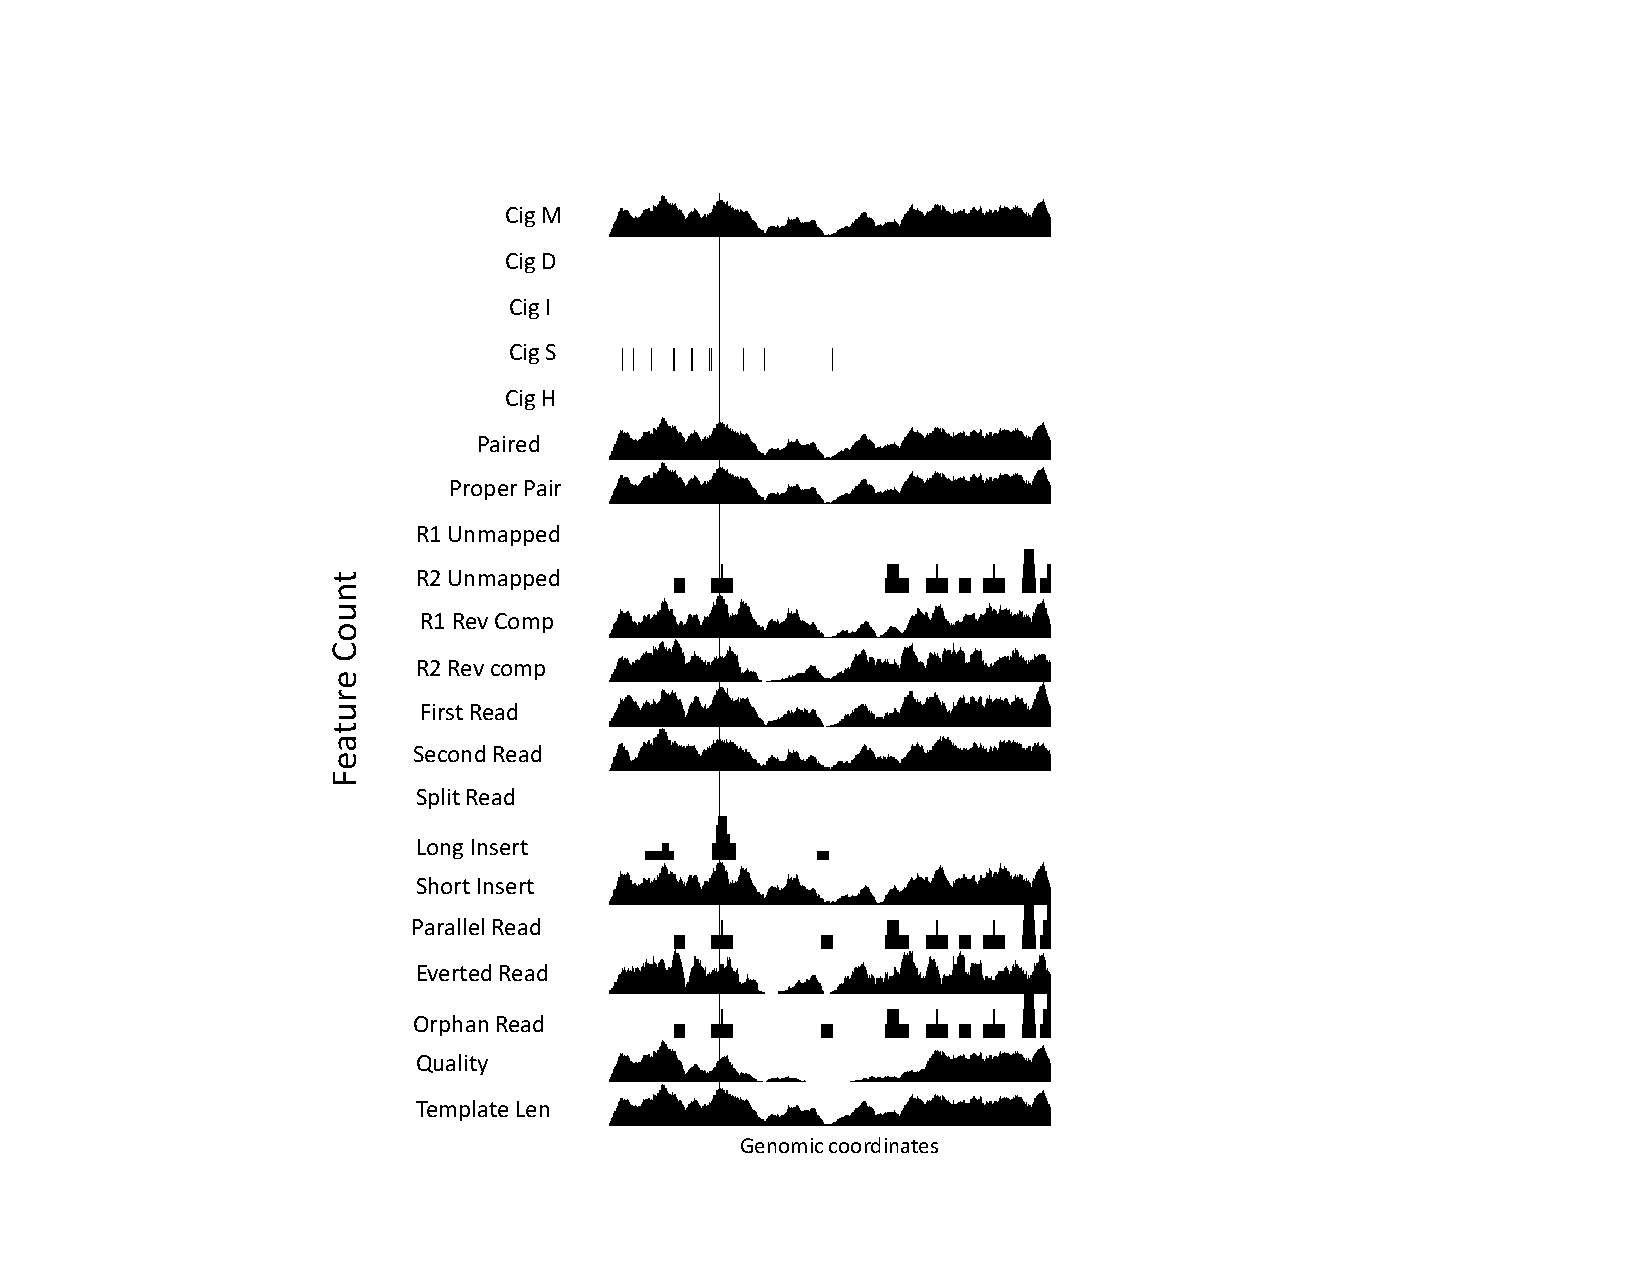
\includegraphics[width=1.5\textwidth]{figures/ch3/example_pileup.pdf}}
    \caption[Sample representations of the object detection feature matrix.]{A representation of the object detection feature matrix. Grey vertical lines represent the left and right breakpoints for a candidate SV region.}
    \label{fig:enter-label}
\end{figure}

